% DANG module details (second architecture figure): (a) Conv-LoRA adapter, (b) token pyramid + scale-aware decoder,
% (c) dual-prototype margin head. Compile: pdflatex figs/arch_modules.tex (standalone, built at full text width).
\documentclass[border=1pt]{standalone}
\usepackage{tikz}
\usepackage{amsmath,amssymb}
\usepackage{graphicx}
\usetikzlibrary{arrows.meta, positioning, fit, backgrounds, calc, shapes.geometric, shapes.misc}

\definecolor{orxblue}{HTML}{0072B2}
\definecolor{orxcyan}{HTML}{56B4E9}
\definecolor{orxorange}{HTML}{E69F00}
\definecolor{ink}{HTML}{333333}

% small snowflake marking frozen weights
\newcommand{\frozen}{\tikz[baseline=-0.55ex]{\foreach \a in {0,60,120}{%
  \draw[orxcyan!90!black, line width=0.5pt, line cap=round] (\a:0.85ex) -- (\a+180:0.85ex);}}}

\tikzset{
  orx/.style={
    font=\sffamily\footnotesize, text=ink,
    >={Stealth[round, length=3.6pt, width=2.8pt]},
    line width=0.55pt,
  },
  block/.style={
    draw=black!50, fill=white, rounded corners=2pt,
    minimum height=10mm, text width=18mm, inner sep=1.8pt, align=center,
  },
  ours/.style={block, draw=orxblue, fill=orxblue!9, line width=0.75pt},
  frozenblk/.style={block, draw=black!35, fill=black!6},
  minor/.style={block, draw=black!40, densely dashed, fill=white, text=black!60},
  encoder/.style={
    draw=black!50, fill=white, trapezium, shape border rotate=270,
    trapezium left angle=72, trapezium right angle=72, trapezium stretches body,
    minimum height=24mm, minimum width=13mm, inner sep=1pt, align=center,
  },
  img/.style={inner sep=0pt, draw=black!40, line width=0.4pt},
  lane/.style={fill=black!3.5, draw=none, rounded corners=3pt, inner xsep=3pt, inner ysep=3pt},
  lanelbl/.style={font=\sffamily\scriptsize\bfseries, text=black!55, inner sep=1pt},
  flow/.style={->, draw=black!65},
  cond/.style={->, densely dashed, draw=orxblue!85},
  edgelbl/.style={font=\scriptsize, text=black!75, inner sep=1.2pt},
  sub/.style={font=\sffamily\scriptsize, text=black!60},
  sumnode/.style={circle, draw=black!65, fill=white, inner sep=0pt, minimum size=4.2mm, font=\small},
}

\tikzset{
  sm/.style={block, minimum height=6.2mm, text width=13mm, inner sep=1.2pt, font=\sffamily\scriptsize},
  smw/.style={sm, text width=19mm},
  smours/.style={sm, draw=orxblue, fill=orxblue!9, line width=0.75pt},
  smfrozen/.style={sm, draw=black!35, fill=black!6},
  tens/.style={font=\scriptsize, text=black!80, inner sep=1pt},
  plabel/.style={font=\sffamily\footnotesize\bfseries, text=ink, anchor=north west, inner sep=0pt},
  ptitle/.style={font=\sffamily\scriptsize, text=black!60, anchor=north west, inner sep=0pt},
  vsum/.style={sumnode, minimum size=3.6mm, font=\scriptsize},
}

\begin{document}
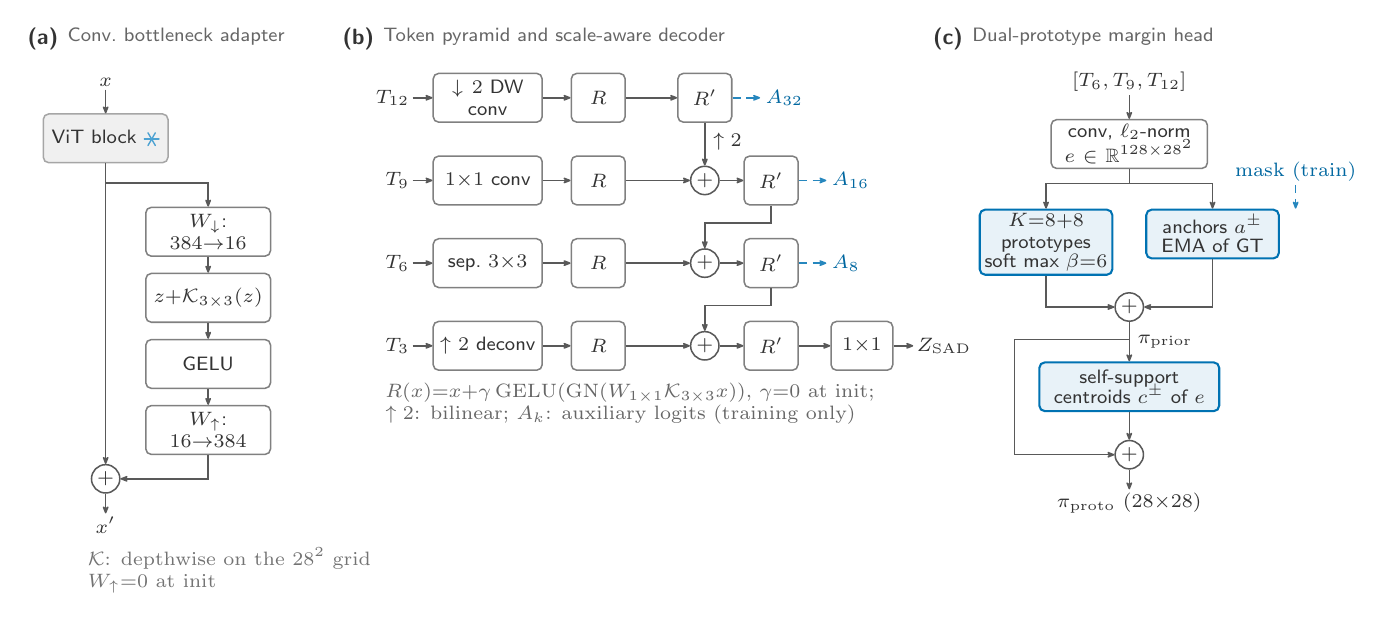
\begin{tikzpicture}[orx, node distance=4.2mm]

  % =============== (a) Conv-LoRA adapter (top to bottom)
  \node[plabel] (la) at (0,0) {(a)};
  \node[ptitle, right=1mm of la.north east, anchor=north west] {Conv.\ bottleneck adapter};
  \node[tens] (xin) at (10mm,-7mm) {$x$};
  \node[smfrozen, below=3mm of xin, text width=15mm] (blk) {ViT block \frozen};
  \coordinate[below=2.5mm of blk] (y);
  \node[sm, anchor=north west, text width=15mm] (down) at ($(y)+(5mm,-3mm)$) {$W_{\downarrow}$: $384{\to}16$};
  \node[sm, below=2mm of down, text width=15mm] (dw) {$z{+}\mathcal{K}_{3\times3}(z)$};
  \node[sm, below=2mm of dw, text width=15mm] (gelu) {GELU};
  \node[sm, below=2mm of gelu, text width=15mm] (up) {$W_{\uparrow}$: $16{\to}384$};
  \node[vsum] (asum) at ($(y |- up.south)+(0,-3mm)$) {$+$};
  \node[tens, below=2.5mm of asum] (xout) {$x'$};
  \draw[flow] (xin) -- (blk);
  \draw[flow] (blk) -- (y) -- (asum);
  \draw[flow] (y) -| (down.north);
  \draw[flow] (down) -- (dw);
  \draw[flow] (dw) -- (gelu);
  \draw[flow] (gelu) -- (up);
  \draw[flow] (up.south) |- (asum.east);
  \draw[flow] (asum) -- (xout);
  \node[tens, text=black!55, anchor=north west, align=left] at ($(xout.south west)+(-1mm,-1mm)$) {$\mathcal{K}$: depthwise on the $28^2$ grid\\$W_{\uparrow}{=}0$ at init};

  % =============== (b) token pyramid + scale-aware decoder (coarse at top, flow downward)
  \node[plabel] (lb) at (40mm,0) {(b)};
  \node[ptitle, right=1mm of lb.north east, anchor=north west] {Token pyramid and scale-aware decoder};
  \node[tens, anchor=east] (t12) at (49mm,-9mm) {$T_{12}$};
  \node[sm, right=2.5mm of t12] (p32) {$\downarrow2$ DW conv};
  \node[sm, right=3.5mm of p32, text width=6mm] (r32) {$R$};
  \node[sm, right=6.5mm of r32, text width=6mm] (q32) {$R'$};
  \foreach \t/\op/\k/\prev [count=\i] in {T_9/{$1{\times}1$ conv}/16/32, T_6/{sep.\ $3{\times}3$}/8/16, T_3/{$\uparrow2$ deconv}/4/8}{
    \node[tens, anchor=east] (t\k) at ($(t12.east)+(0,-\i*10.5mm)$) {$\t$};
    \node[sm, right=2.5mm of t\k] (p\k) {\op};
    \node[sm, right=3.5mm of p\k, text width=6mm] (r\k) {$R$};
    \node[vsum] (s\k) at (q32 |- r\k) {$+$};
    \node[sm, right=3mm of s\k, text width=6mm] (q\k) {$R'$};
    \draw[flow] (t\k) -- (p\k);
    \draw[flow] (p\k) -- (r\k);
    \draw[flow] (r\k) -- (s\k);
    \draw[flow] (s\k) -- (q\k);
  }
  \draw[flow] (t12) -- (p32);
  \draw[flow] (p32) -- (r32);
  \draw[flow] (r32) -- (q32);
  \draw[flow] (q32.south) -- node[tens, right=0.6mm, pos=0.45] {$\uparrow2$} (s16.north);
  \draw[flow] (q16.south) -- ++(0,-2.2mm) -| (s8.north);
  \draw[flow] (q8.south) -- ++(0,-2.2mm) -| (s4.north);
  \node[sm, right=4mm of q4, text width=7mm] (o4) {$1{\times}1$};
  \node[tens, right=2.5mm of o4] (zsad) {$Z_{\mathrm{SAD}}$};
  \draw[flow] (q4) -- (o4);
  \draw[flow] (o4) -- (zsad);
  \foreach \k in {32,16,8}{ \draw[cond] (q\k.east) -- ++(3.5mm,0) node[tens, right=0.3mm, text=orxblue!90!black] {$A_{\k}$}; }
  \node[tens, text=black!60, anchor=north west, align=left] at ($(t4.south west)+(0,-2.8mm)$)
       {$R(x){=}x{+}\gamma\,\mathrm{GELU}(\mathrm{GN}(W_{1\times1}\mathcal{K}_{3\times3}x))$, $\gamma{=}0$ at init;\\$\uparrow2$: bilinear; $A_k$: auxiliary logits (training only)};

  % =============== (c) dual-prototype margin head (top to bottom)
  \node[plabel] (lc) at (115mm,0) {(c)};
  \node[ptitle, right=1mm of lc.north east, anchor=north west] {Dual-prototype margin head};
  \node[tens] (tin) at (140mm,-7mm) {$[T_6,T_9,T_{12}]$};
  \node[smw, below=3mm of tin] (emb) {conv, $\ell_2$-norm\\[-1pt]$e\in\mathbb{R}^{128\times28^2}$};
  \node[smours, below left=5mm and -8mm of emb, text width=16mm] (bank) {$K{=}8{+}8$ prototypes\\[-1pt]soft max $\beta{=}6$};
  \node[smours, below right=5mm and -8mm of emb, text width=16mm] (anch) {anchors $a^{\pm}$\\[-1pt]EMA of GT};
  \node[vsum] (psum) at ($(bank.south)!0.5!(anch.south)+(0,-5mm)$) {$+$};
  \node[smours, below=5mm of psum, text width=22mm] (ss) {self-support\\[-1pt]centroids $c^{\pm}$ of $e$};
  \node[vsum, below=3.5mm of ss] (fsum) {$+$};
  \node[tens, below=2.5mm of fsum] (pout) {$\pi_{\mathrm{proto}}$ ($28{\times}28$)};
  \draw[flow] (tin) -- (emb);
  \draw[flow] (emb.south) -- ++(0,-1.8mm) -| (bank.north);
  \draw[flow] (emb.south) -- ++(0,-1.8mm) -| (anch.north);
  \draw[flow] (bank.south) |- (psum.west);
  \draw[flow] (anch.south) |- (psum.east);
  \draw[flow] (psum) -- node[tens, right=0.6mm] {$\pi_{\text{prior}}$} (ss);
  \draw[flow] (ss) -- (fsum);
  \coordinate (pp) at ($(psum.south)!0.45!(ss.north)$);
  \draw[flow] (pp) -| ($(ss.west)+(-3mm,0)$) |- (fsum.west);
  \draw[flow] (fsum) -- (pout);
  \draw[cond] ($(anch.north east)+(2mm,3mm)$) node[tens, anchor=south, text=orxblue!90!black] {mask (train)} -- ($(anch.north east)+(2mm,0)$);

\end{tikzpicture}
\end{document}
